\chapter{Preliminaries}
\label{sec:preliminaries}

Before introducing the formal details of the new automaton model at the heart of this thesis, this chapter establishes the necessary theoretical foundation. We will review the standard definitions and notations from formal language theory, focusing on Deterministic Finite Automata (DFAs) as the canonical model for regular languages. Furthermore, we will define Deterministic Generalized Automata (DGAs), a key model for comparison that also utilizes strings on transitions but with a strict prefix-based matching rule. This groundwork will provide the precise vocabulary and context required to properly situate and analyze the novel suffix-reading paradigm presented in the chapters that follow.

We fix a finite alphabet $\Sigma$. Following standard convention, we
write $\Sigma^*$ for the set of all words (including $\e$) over
$\Sigma$, and $\Sigma^+ = \Sigma^* \setminus \{ \e\}$. For
$w \in \Sigma^*$, we write $|w|$ for the length of $w$, with $|\e|$
considered to be $0$.  A word $u$ is a \emph{prefix} of word $w$ if
$w = u v$ for some $v \in \Sigma^*$; it is a \emph{proper-prefix} if
$v \in \Sigma^+$. Observe that $\e$ is a prefix of every word. A set
of words $W$ is said to be a \emph{prefix-free set} if no word in $W$
is a prefix of another word in $W$. A word $u$ is a
\emph{suffix} (resp. \emph{proper-suffix}) of $w$ if $w = vu$ for some
$v \in \Sigma^*$ (resp. $v \in \Sigma^+$).

A \emph{Deterministic Finite Automaton (DFA)} $M$ is a tuple
$(Q, \Sigma, q^{init}, \delta, F)$ where $Q$ is a finite set of
states, $q^{init} \in Q$ is the initial state, $F \incl Q$ is a set of
accepting states, and $\delta: Q \times \Sigma \to Q$ is a partial
function describing the transitions. If $\delta$ is complete, the
automaton is said to be a complete DFA. Else, it is called a trim
DFA. The run of DFA $M$ on a word $w = a_1 a_2 \dots a_n$ (where
$a_i \in \Sigma$) is a sequence of transitions
$(q_0, a_1, q_1) (q_1, a_2, q_2) \dots (q_{n-1}, a_n, q_n)$ where $\delta(q_i, a_{i+1}) = q_{i+1}$ for each $0 \le i < n$, and
$q_0 = q^{init}$, the initial state of $M$. The run is accepting if
$q_n \in F$. If the DFA is complete, every word has a unique run. On a
trim DFA, each word either a has unique run, or it has no run. The
language $\Ll(M)$ of DFA $M$, is the set of words for which $M$ has an
accepting run.

We will now recall some useful facts about minimality of DFAs. Here,
by minimality, we mean DFAs with the least number of states. Every
complete DFA $M$ induces an equivalence $\sim_M$ over words:
$u \sim_M v$ if $M$ reaches the same state on reading both $u$ and $v$
from the initial state.  In the case of trim DFAs, this equivalence
can be restricted to set of prefixes of words in $\Ll(M)$. For a
regular language $L$, we have the Nerode equivalence: $u \approx_L v$
if for all $w \in \Sigma^*$, we have $uw \in L$ iff $v w \in L$. By
the well-known Myhill-Nerode theorem (see
\cite{DBLP:books/daglib/0016921} for more details), there is a
canonical DFA $M_L$ with the least number of states for $L$, and
$\sim_{M_L}$ equals the Nerode equivalence $\approx_L$. Furthermore,
every DFA $M$ for $L$ is a \emph{refinement} of $M_L$: $u \sim_M v$
implies $u \sim_{M_L} v$. If two words reach the same state in $M$,
they reach the same state in $M_L$.


  A \emph{Deterministic Generalized Automaton (DGA)}~\cite{giammarresi1999deterministic} $H$ is given by
  $(Q, \Sigma, q^{init}, E, F)$ where $Q, q^{init}, F$ mean the same
  as in DFA, and $E \incl Q \times \Sigma^+ \times Q$ is a finite set
  of edges labeled with words from $\Sigma^+$. For every state $q$,
  the set $\{ \alpha \mid (q, \alpha, q') \in E \}$ is a prefix-free
  set.
A run of DGA $H$ on a word $w$ is a sequence of edges
$(q_0, \alpha_1, q_1) (q_1, \alpha_2, q_2) \dots (q_{n-1}, \a_n, q_n)$
such that $w = \alpha_1 \alpha_2 \dots \a_n$, with $q_0$ being the
initial state. As usual, the run is accepting if $q_n \in F$. Due to
the property of the set of outgoing labels being a prefix-free set,
there is a atmost one run on every word. The language $\Ll(H)$ is the
set of words with an accepting run. Figure~\ref{fig:dfa-dga-examples}
gives examples of DFAs and corresponding DGAs.

\begin{figure}
  \centering
  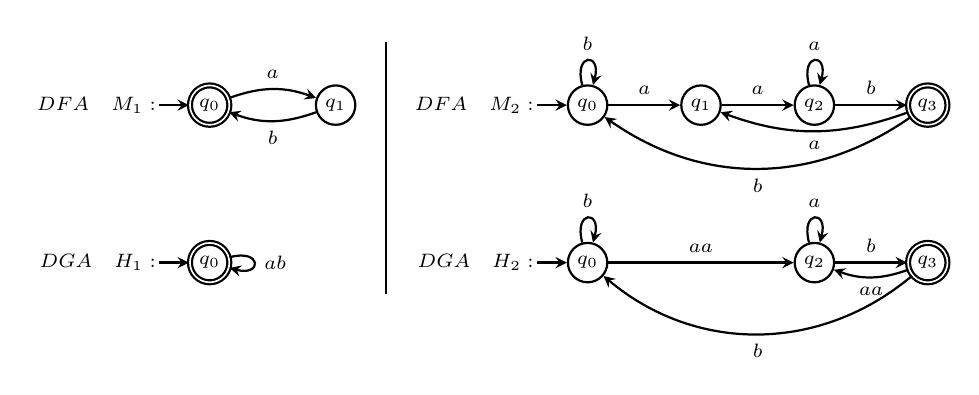
\begin{tikzpicture}[state/.style={circle, draw, thick, inner sep =
      2pt}, scale=0.8]
    \begin{scope}[every node/.style={state}]
      \node [double] (0) at (0,0) {\scriptsize $q_0$}; \node (1) at
      (2,0) {\scriptsize $q_1$};
    \end{scope}
    \begin{scope}[->,>=stealth, thick, auto]
      \draw (-0.8, 0) to (0); \draw (0) to [bend left=20] node
      {\scriptsize $a$} (1); \draw (1) to [bend left=20] node
      {\scriptsize $b$} (0);
    \end{scope}
    \node [left] at (-0.7, 0) {\scriptsize $DFA \quad M_1:$};

    \begin{scope}[yshift=-2.5cm]
      \begin{scope}[every node/.style={state}]
        \node [double] (0) at (0,0) {\scriptsize $q_0$};
      \end{scope}
      \begin{scope}[->,>=stealth, thick, auto]
        \draw (-0.8, 0) to (0); \draw (0) to [loop right] node
        {\scriptsize $ab$} (0);
      \end{scope}
      \node [left] at (-0.7, 0) {\scriptsize $DGA \quad H_1:$};
    \end{scope}

    \draw (2.8,-3) to (2.8,1);
    
    \begin{scope}[xshift = 6cm]
      \begin{scope}[every node/.style={state}]
        \node (0) at (0,0) {\scriptsize $q_0$}; \node (1) at (1.8,0)
        {\scriptsize $q_1$}; \node (2) at (3.6,0) {\scriptsize $q_2$};
        \node [double] (3) at (5.4,0) {\scriptsize $q_3$};
      \end{scope}

      \begin{scope}[->,>=stealth, thick, auto]
        \draw (-0.8, 0) to (0); \draw (0) to [loop above] node
        {\scriptsize $b$} (0); \draw (0) to node {\scriptsize $a$}
        (1); \draw (1) to node {\scriptsize $a$} (2); \draw (2) to
        [loop above] node {\scriptsize $a$} (2); \draw (2) to node
        {\scriptsize $b$} (3); \draw (3) to [bend left=20] node
        {\scriptsize $a$} (1); \draw (3) to [bend left=35] node
        {\scriptsize $b$} (0);
       
      \end{scope}
      \node [left] at (-0.7, 0) {\scriptsize $DFA \quad M_2:$};

      \begin{scope}[yshift=-2.5cm]
        \begin{scope}[every node/.style={state}]
          \node (0) at (0,0) {\scriptsize $q_0$}; \node (2) at (3.6,0)
          {\scriptsize $q_2$}; \node [double] (3) at (5.4,0)
          {\scriptsize $q_3$};
        \end{scope}
        \begin{scope}[->,>=stealth, thick, auto]
          \draw (-0.8, 0) to (0); \draw (0) to [loop above] node
          {\scriptsize $b$} (0); \draw (0) to node {\scriptsize $aa$}
          (2); \draw (2) to [loop above] node {\scriptsize $a$} (2);
          \draw (2) to node {\scriptsize $b$} (3); \draw (3) to [bend
          left=20] node {\scriptsize $aa$} (2); \draw (3) to [bend
          left=40] node {\scriptsize $b$} (0);
       
      \end{scope}
      \node [left] at (-0.7, 0) {\scriptsize $DGA \quad H_2:$};
    \end{scope}
  \end{scope}
 
\end{tikzpicture}
\caption{Examples of DFAs and corresponding DGAs, over alphabet
  $\{a, b\}$.}
\label{fig:dfa-dga-examples}
\end{figure}


It was
shown in~ \cite{giammarresi1999deterministic} that there is no unique smallest DGA. The paper defines an operation
to suppress states and create longer labels. A state of a DGA is
called \emph{superflous} if it is neither the initial nor final state,
and it has no self-loop. For example, in
Figure~\ref{fig:dfa-dga-examples}, in $M_1$ and $M_2$, state $q_1$ is
superfluous. Such states can be removed, and every pair
$p \xra{\alpha} q$ and $q \xra{\beta} r$ can be replaced with
$p \xra{\alpha \beta} r$.  This operation is extended to a set of
states: given a DGA $H$, a set of states $S$, a DGA $\Ss(H, S)$ is
obtained by suppressing states of $S$, one after the other, in any
arbitrary order. For correctness, there should be no cycle in the
induced subgraph of $H$ restricted to $S$.
The paper proves that minimal DGAs (in number of
states) can be derived by suppressing states, starting from the
canonical DFA.









\section{Automata models in Practical applications}

Deterministic Finite Automata (DFAs) are a cornerstone of computer science, serving as a fundamental model in both theoretical and practical domains. Beyond their foundational role in the study of regular languages, they have been widely applied in areas as diverse as text processing~\cite{DBLP:journals/tcs/MohriMW09}, formal specification languages~\cite{DBLP:journals/scp/Harel87}, and as the underlying engine for verification techniques like model-checking~\cite{DBLP:books/daglib/0007403-2} and runtime verification~\cite{DBLP:conf/cav/BouajjaniJNT00, DBLP:conf/cav/BouajjaniHV04, 989841}. The broad utility of automata is further evidenced by the development of numerous software libraries dedicated to their creation and manipulation~\cite{Awali2.2}.

However, a central challenge consistently hinders their practical application: the state-space explosion problem. Although the state-and-transition paradigm is intuitive, its descriptions operate at a low level of abstraction. This granular, character-by-character processing often results in automata of unmanageable size for non-trivial applications, creating a persistent need for more concise formalisms. While non-determinism is a well-known path to exponential succinctness, a deterministic model is often essential for unambiguous formal specifications and efficient automata implementations. The following survey discusses several deterministic approaches from the literature aimed at tackling this problem of large DFA size.

One major strategy for achieving succinctness is to enhance transition labels, moving from single letters to more complex patterns. \emph{Generalized automata} (GA), first defined by Eilenberg~\cite{DBLP:books/lib/Eilenberg74}, extend non-deterministic automata with string-labeled transitions; a word is accepted if it can be partitioned into segments that match a sequence of these transition labels. Subsequent work established bounds on the label lengths required for minimal GAs~\cite{DBLP:conf/icalp/Hashiguchi91}. The deterministic variant, \emph{Deterministic Generalized Automata} (DGA), requires that for any state, the set of outgoing string labels must be prefix-free~\cite{giammarresi1999deterministic}. The key method for constructing smaller DGAs involves starting with a DFA and "suppressing" states to create longer labels. Giammarresi et al.~\cite{giammarresi1999deterministic} showed that minimal DGAs (in terms of state count) can be derived from the canonical DFA using this technique. However, the more natural question of minimizing the \emph{total size} of a DGA—a metric that includes the number of states, edges, and the sum of label lengths—was left as an open problem. A natural extension from strings to more complex objects is to consider regular expressions. The resulting model, known as \emph{Expression Automata}~\cite{DBLP:conf/wia/HanW04}, was first considered in the context of converting automata to regular expressions~\cite{DBLP:journals/tc/BrzozowskiM63}. To achieve determinism, however, the \emph{Deterministic Expression Automata} (DEA) model imposes two strict requirements: from any state, the languages of any two outgoing expressions must be disjoint, and each of those languages must be prefix-free. This latter restriction makes DEAs less expressive than standard DFAs, as they are unable to recognize any regular language that is not prefix-free.

Another strategy for succinctness targets complexity that arises from the size of the alphabet itself. For instance, an alphabet consisting of all ASCII characters can cause the number of transitions to blow up. \emph{Symbolic automata}~\cite{DBLP:conf/popl/VeanesHLMB12, DBLP:conf/cav/DAntoniV17} have been proposed to handle large or infinite alphabets. They replace letters on edges with logical formulas or predicates, which allows them to club together numerous transitions between a pair of states into a single symbolic transition. For example, if the domain is the set of natural numbers, a transition labeled with a predicate like $\operatorname{odd(x)}$ can act as a placeholder for all transitions labeled with an odd number~\cite{loris-page}. This approach has been widely applied and implemented in many tools~\cite{loris-page}.

Despite these advances, a gap remains for a formalism that can succinctly model behaviors defined by high-level patterns that are not necessarily contiguous prefixes and may be separated by long, irrelevant sequences of events.

\paragraph*{Our model.} In this work, we introduce \emph{Deterministic Suffix-reading Automata (DSAs)} to fill this gap. We continue to work with strings on transitions, as in a DGA. However, the meaning of transitions is different. A transition $q \xra{abba} q'$ is enabled if at $q$, a word $w$ \emph{ending} with $abba$ is seen, and moreover no other transition out of $q$ is enabled at any proper prefix of $w$. Intuitively, the automaton tracks a finite set of pattern strings at each state. It stays in a state, passively consuming input, until one of them appears as the \emph{suffix} of the word read so far, and then makes the appropriate transition.

We start with a motivating example. Consider a model for out-of-context \texttt{else} statements, in relation to \texttt{if} and \texttt{endif} statements in a programming language. Assume a suitable alphabet $\Sigma$ of characters. Let $L_{\texttt{else}}$ be the set of all strings over the alphabet where (1) there are no nested \texttt{if} statements, and (2) there is an \texttt{else} which is not between an \texttt{if} and an \texttt{endif}. A standard DFA for this language would need to perform detailed string matching to detect the keywords. The DSA, shown in Figure~\ref{fig:if-else}, offers a more direct abstraction. At state $s_0$, it passively reads letters until it first sees a suffix matching either \texttt{if} or \texttt{else}. If the first match is \texttt{if}, it transitions to $s_1$. For instance, on a word like \texttt{abf4fgif}, the automaton moves to $s_1$ because the word ends with \texttt{if} and no trigger pattern appeared in any of its proper prefixes. Similarly, from $s_1$, it waits for the next pattern, \texttt{if} or \texttt{endif}, to decide its next move.

Suffix-reading automata have the ability to wait at a state, reading long words until a matching pattern is seen. This results in an arguably more readable specification for languages which are ``pattern-intensive''. This representation is orthogonal to the approaches considered so far. While symbolic automata club together transitions between a specific pair of states, DSAs can consolidate entire paths of states and transitions. And while DGAs can also club paths, they cannot ignore intermediate letters, which can result in extra states and transitions that DSAs can avoid.
%%% Local Variables:
%%% mode: latex
%%% TeX-master: "dsa-main"
%%% End:









\begin{figure}[t]
  \centering
  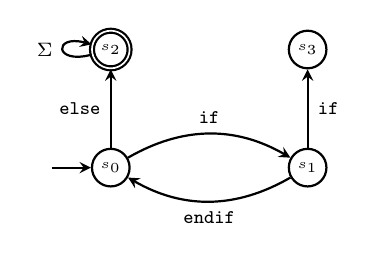
\begin{tikzpicture}[state/.style={circle, draw, thick, inner sep =
      2pt}]
    \begin{scope}[every node/.style={state}]
      \node (0) at (0,0) {\tiny $s_0$}; \node (1) at (2.5, 0) {\tiny
        $s_1$}; \node [double] (2) at (0, 1.5) {\tiny $s_2$}; \node
      (3) at (2.5, 1.5) {\tiny $s_3$};
    \end{scope}
    \begin{scope}[->, >=stealth, thick, auto]
      \draw (-0.75, 0) to (0); \draw (0) to node {\scriptsize
        $\mathtt{else}$ } (2); \draw (0) to [bend left=30] node
      {\scriptsize $\mathtt{if}$} (1); \draw (1) to [bend left=30]
      node {\scriptsize $\mathtt{endif}$} (0); \draw (2) to [loop
      left] node {\scriptsize $\Sigma$} (2); \draw (1) to node [right]
      {\scriptsize $\mathtt{if}$} (3);
    \end{scope}
  \end{tikzpicture}
  \caption{DSA for out-of-context \texttt{else}}
  \label{fig:if-else}
\end{figure}



\paragraph*{Overview of results.}
We formally present deterministic suffix-reading automata and its
semantics, quantify its size in comparison to an equivalent DFA, and
study an algorithm to construct DSAs starting from a DFA. This is in
the same spirit as in DGAs, where smaller DGAs are obtained by suppressing
states. For automata models with strings on transitions, the number of
states is not a faithful measure of the size of a DSA. As described
in~\cite{giammarresi1999deterministic} for DGAs, we consider the total-size of
a DSA which includes the number of states, edges, and the sum of label
lengths. The key contributions of this paper are:
\begin{enumerate}
\item Presentation of a definition of a new kind of automaton - DSA~(Chapter~\ref{sec:new-automaton-model}).

\item Proof that DSAs accept regular languages, and nothing more.
  Every complete DFA can be seen as a DSA. For the converse, we prove
  that for every DSA of size $k$, there is a DFA with size at most
  $2k \cdot (1 + 2 |\Sigma|)$, where $\Sigma$ is the alphabet
  (Lemma~\ref{lem:tracking-dfa-language-equivalent},
  Theorem~\ref{thm:comparing-dsa-with-dfa-dga}).
  This answers the question of how small DSAs can be in comparison to
  DFAs for a certain language : if $n$ is the size of the minimal DFA
  for a language $L$, minimal DSAs for $L$ cannot be smaller than
  $\frac{n}{2 \cdot (1 + 2
    |\Sigma|)}$. 
  When the alphabet is large, one could expect smaller sized DSAs. We
  describe a family of languages $L_n$, with alphabet size $n$, for
  which the minimal DFA has size quadratic in $n$, whereas size of
  DSAs is a linear function of $n$ (Lemma~\ref{lem:dsa-small}).

\item We present a method to derive DSAs out of DFAs, a DFA-to-DSA
  conversion (Chapter~\ref{sec:suffix-tracking-sets}). In a nutshell,
  the derivation procedure selects subsets of DFA-states, and adds
  transitions labeled with (some of) the acyclic paths between
  them. Our main
  technical contribution lies in identifying sufficient conditions on
  the selected subset of states, so that the derivation procedure
  preserves the language (Theorem~\ref{def:suffix-tracking-set}).

\item We remark that minimal DSAs need not be unique, and make a
  surprising observation: the smallest DSA that we derive from the
  canonical DFA of a language $L$ need not be a minimal DSA. We find this
  surprising because (1) firstly, our derivation procedure is
  surjective: every DSA (satisfying some natural assumptions) can be
  derived from some corresponding DFA, and in particular, a minimal
  DSA can be derived from some DFA; (2) the observation suggests that
  one may need to start with a bigger DFA in order to derive a minimal
  DSA -- so, starting with a bigger DFA may result in a smaller DSA
  (Section~\ref{sec:minim-some-observ}).

\item Inspired by the above observation, we present a restriction to the definition of DSA, called \emph{strong DSA} (Section~\ref{sec:strong}). We show that minimal strong DSAs can in fact be derived from the canonical DFA, through our derivation procedure. 


\item Finally, we show that given a DFA and a number $k$, deciding if
  there exists a DSA of size $\le k$ is $\NP$-complete
  (Section~\ref{sec:complexity}).

\end{enumerate}

This chapter has provided the necessary formal preliminaries, defining the classical DFA model and the closely related DGA. With this foundational framework in place, we have established a common language and a basis for comparison. We are now prepared to move from these traditional prefix-matching models to the central contribution of this work. The following chapter will introduce the Deterministic Suffix-reading Automaton (DSA), presenting its formal syntax, its unique suffix-based operational semantics, and an initial analysis of its expressive power and succinctness.

\paragraph*{Related work.} The closest to our work
is~\cite{giammarresi1999deterministic} which introduces DGAs, and
gives a procedure to derive DGAs from DFAs. The focus however is on
getting DGAs with as few states as possible. The observations presented in
Chapter~\ref{sec:minim-some-observ} of our work, also apply for
state-minimality: the same example shows that in order to get a DSA with fewer
states, one may have to start with a bigger DFA.  This is in sharp
contrast to the DGA setting, where the derivation procedure of
\cite{giammarresi1999deterministic} yields a minimal DGA (in the
number of states) when applied on the canonical DFA. The problem of
deriving DGAs with minimal total-size was left open
in~\cite{giammarresi1999deterministic}, and continues to remain so, to
the best of our knowledge.
Expression automata~\cite{DBLP:conf/wia/HanW04} allow regular
expressions as transition labels.  This model was already considered
in~\cite{DBLP:journals/tc/BrzozowskiM63} to convert automata to
regular expressions. Every DFA can be converted to a two state
expression automaton with a regular expression connecting them.  A
model of deterministic Expression automata (DEA) was proposed
in~\cite{DBLP:conf/wia/HanW04} with restrictions that limit the
expressive power.  An algorithm to convert a DFA to a DEA, by repeated
state elimination, is proposed in~\cite{DBLP:conf/wia/HanW04}. The
resulting DEA is minimal in the number of states.  
Minimization of NFAs was studied
in~\cite{DBLP:journals/siamcomp/JiangR93} and shown to be
hard. Succinctness of models with different features, like alternation,
two-wayness, pebbles, and a notion of concurrency, has been studied
in~\cite{DBLP:journals/tcs/GlobermanH96}.

Here are some works that are related to the spirit of finding more readable specifications. \cite{fernau2009algorithms} has used the model of deterministic GA to
develop a learning algorithm for some simple forms of regular
expressions, with
applications in learning DTD specifications for XML code. In this
paper, the author talks about readability of specifications. They
claim that regular expressions (REs) are arguably the best way to
specify regular 
languages. They also claim that the translation algorithms from DFAs
to REs give unreadable REs. In the paper, they consider specific
language classes and generate algorithms to learn simple looking REs.

Another work that talks about readability of specifications
is~\cite{DBLP:conf/icse/ZimmermanLL02}. They consider automata based
specification languages and perform extensive
experiments to determine which choice of syntax gives better
readability. They remark that hierarchical specifications are easier,
since not every transition needs to be specified. Once again, we
observe that there is an effort to remove transitions. Another
formalism is proposed in~\cite{DBLP:conf/date/VenkateshSKA14} which
uses a tabular notation where each cell contains patterns, which is
then compiled into a usual automaton for analysis.







%%% Local Variables:
%%% mode: latex
%%% TeX-master: "dsa-main"
%%% End:

